\chapter{Cadre Général du Projet}
	
	\section*{Introduction}
	\addcontentsline{toc}{section}{Introduction}
	
Ce chapitre pose les fondements contextuels indispensables à la compréhension de la portée et des ambitions du HydroNova. Il s'ouvre sur la présentation de MicroEdition, l'organisme d'accueil, en détaillant son positionnement stratégique dans le domaine de l'intelligence embarquée et des écosystèmes IoT industriels. Nous procédons ensuite à une analyse critique du paysage technologique agricole actuel, en identifiant les lacunes structurelles des solutions disponibles sur le marché. Cette analyse nous permet de justifier la pertinence et la valeur ajoutée de notre système proposé. Le chapitre s'achève par la présentation de la méthodologie en Cycle en V, cadre d'ingénierie retenu pour structurer l'ensemble du processus de développement et de validation.
	
	%----------------------------------------------------------------
	\section{Présentation de l'organisme d'accueil}
	%----------------------------------------------------------------
	
	\subsection{Profil de l'entreprise et vision stratégique}
	
Fondée en 2025 et implantée au sein de la Pépinière d'Entreprises de Mahdia, MicroEdition est une entreprise technologique  spécialisée dans les Technologies de l'Information et de la Communication. Sa vocation fondatrice est de combler le fossé entre la recherche académique avancée et les solutions industrielles directement déployables sur le terrain.
L'intégration au sein de la pépinière offre à l'entreprise un écosystème collaboratif particulièrement stimulant: accès à une infrastructure technique adaptée au prototypage rapide, à un réseau interdisciplinaire de partenaires académiques et industriels, et à un environnement propice à l'expérimentation à moindre risque. Cette proximité avec la recherche constitue un atout déterminant pour mener des projets à forte composante d'innovation, comme le HydroNova.
	
	\subsectiontitle{Piliers technologiques centraux}
	
	Le portefeuille opérationnel de MicroEdition s'articule autour de trois domaines d'expertise profondément interconnectés :
	
	\begin{itemize}
		\item \textbf{Ingénierie Logicielle: } L'entreprise conçoit des architectures logicielles modulaires et évolutives, ainsi que des interfaces utilisateurs multiplateformes et réactives. L'accent est mis sur la maintenabilité, la testabilité et la scalabilité des systèmes produits, afin de garantir une évolution fluide et durable des solutions développées.
		
		\item \textbf{Internet des Objets Industriel (IIoT): } MicroEdition développe des réseaux embarqués résilients capables d'orchestrer des interactions matérielles autonomes. Ces réseaux s'appuient sur des protocoles de communication légers et sur des processus déterministes, garantissant la fiabilité des échanges même dans des environnements contraints en bande passante ou soumis à des coupures réseau fréquentes.
		
		\item \textbf{Intelligence Artificielle Embarquée (Edge AI): } Le déploiement de modèles de Machine Learning directement sur des dispositifs à ressources limitées constitue la compétence différenciante de l'entreprise. Cette approche dite Edge-first élimine la latence et les risques d'indisponibilité inhérents à l'inférence basée sur le Cloud, tout en préservant la confidentialité des données produites localement.
	\end{itemize}
	\subsectiontitle{Dynamique Organisationnelle et R\&D}
	
	L'entreprise adopte une organisation hybride des processus de développement, adaptée à la nature des projets et à leurs contraintes spécifiques. Cette approche combine des cycles structurés de type prédictif pour les phases critiques, et des pratiques itératives inspirées des méthodes Agiles afin de favoriser la flexibilité, la réactivité et l'amélioration continue.
	
	La cellule dédiée à la Recherche et Développement (R\&D) est concentrée sur l'optimisation des contraintes de calcul des dispositifs "Edge" (à la périphérie du réseau). Cette compétence en R\&D a été un facteur déterminant pour le système \textit{HydroNova}, fournissant l'expertise requise pour exécuter des réseaux de neurones convolutifs directement sur un Raspberry Pi déployé localement.
	%----------------------------------------------------------------
%----------------------------------------------------------------
\section{Contexte général du projet}
%----------------------------------------------------------------

L’agriculture connaît aujourd’hui une transformation profonde sous l’effet de la révolution numérique. Face à la croissance démographique mondiale, à la raréfaction des ressources naturelles et aux changements climatiques, les méthodes agricoles traditionnelles montrent certaines limites en matière de productivité, de gestion des ressources et de résilience environnementale. Dans ce contexte, l’intégration des technologies numériques dans les systèmes agricoles apparaît comme une solution prometteuse pour améliorer l’efficacité des exploitations tout en garantissant une utilisation plus rationnelle des ressources.

Cette évolution a donné naissance au concept d’\textit{Agriculture 4.0}, qui repose sur l’exploitation des technologies de l’Internet des Objets , de l’Intelligence Artificielle , du Cloud Computing et de l’analyse des données afin de moderniser les pratiques agricoles. L’objectif est de transformer les exploitations agricoles en systèmes intelligents capables de collecter, analyser et exploiter les données en temps réel pour optimiser la prise de décision et automatiser les processus de production.

%----------------------------------------------------------------
\subsection{Agriculture intelligente et Agriculture 4.0}
%----------------------------------------------------------------

L’Agriculture 4.0 représente l’application des technologies numériques avancées au secteur agricole. Elle vise à améliorer la productivité, réduire les coûts d’exploitation et limiter l’impact environnemental des activités agricoles grâce à une gestion intelligente des ressources.

L’un des piliers fondamentaux de cette transformation est l’Internet des Objets. Les capteurs connectés permettent de mesurer en temps réel différents paramètres tels que la température, l’humidité, la luminosité, le pH ou encore la qualité de l’eau. Ces données sont ensuite transmises vers des plateformes de supervision capables de surveiller l’état des cultures et de déclencher automatiquement des actions correctives lorsque cela est nécessaire.

Parallèlement, l’Intelligence Artificielle joue un rôle croissant dans l’automatisation des tâches agricoles. Grâce aux techniques d’apprentissage automatique et de vision par ordinateur, il devient possible de détecter précocement certaines maladies végétales, d’identifier des anomalies de croissance ou encore de fournir des recommandations adaptées aux agriculteurs. Ces technologies contribuent à améliorer la qualité de la production tout en réduisant les interventions manuelles.

Enfin, les systèmes de supervision connectée offrent une visibilité globale sur l’exploitation agricole. Les données collectées par les capteurs peuvent être visualisées à travers des applications mobiles ou des interfaces web, permettant aux utilisateurs de suivre l’évolution des paramètres environnementaux, de recevoir des alertes en temps réel et de piloter les équipements à distance. Cette approche favorise une gestion plus réactive, plus précise et davantage orientée vers l’optimisation des performances.

%----------------------------------------------------------------
\subsection{Hydroponie et production de fourrage}
%----------------------------------------------------------------

Parmi les approches innovantes adoptées dans le cadre de l’agriculture intelligente, l’hydroponie occupe une place importante. Cette technique consiste à cultiver les plantes sans sol, en utilisant une solution nutritive contrôlée qui fournit directement aux racines les éléments nécessaires à leur développement. Grâce à la maîtrise des conditions de culture, l’hydroponie permet d’obtenir une croissance rapide et régulière tout au long de l’année.

Dans le domaine de l’élevage, la production de fourrage hydroponique constitue une alternative intéressante aux méthodes conventionnelles. Les graines, généralement de l’orge, sont placées dans des plateaux de culture et irriguées de manière contrôlée pendant plusieurs jours jusqu’à obtenir un tapis végétal riche en nutriments destiné à l’alimentation animale. Ce procédé permet de produire du fourrage frais en continu, indépendamment des conditions climatiques extérieures.

L’hydroponie présente plusieurs avantages significatifs. Elle permet notamment une réduction importante de la consommation d’eau, une optimisation de l’espace de production, une diminution de la dépendance aux terres agricoles ainsi qu’une meilleure maîtrise des paramètres environnementaux. De plus, la production peut être réalisée de manière continue, garantissant une disponibilité régulière du fourrage pour les exploitations d’élevage.

Cependant, cette méthode présente également certaines contraintes. Les cultures hydroponiques nécessitent un contrôle permanent des paramètres environnementaux tels que la température, l’humidité, l’éclairage et les cycles d’irrigation. Une défaillance technique ou une variation importante de ces paramètres peut affecter rapidement la qualité de la production. Par ailleurs, les environnements humides favorisent le développement de maladies et de moisissures, rendant indispensable la mise en place de mécanismes de surveillance et de détection précoce.

C’est dans cette perspective que s’inscrit notre projet, dont l’objectif est de concevoir une serre hydroponique intelligente reposant sur l’intégration de technologies IoT, d’algorithmes d’Intelligence Artificielle et d’interfaces de supervision connectées afin d’automatiser la production, d’améliorer la surveillance des cultures et d’optimiser l’utilisation des ressources.
\section{Présentation du problème}
%----------------------------------------------------------------

L’agriculture moderne fait face à de nombreux défis qui impactent directement la productivité des exploitations et la sécurité alimentaire. Dans le contexte tunisien, ces difficultés concernent aussi bien les aspects agricoles que les aspects technologiques. La mise en place d’un système hydroponique intelligent nécessite donc de répondre simultanément à ces deux catégories de contraintes.

%----------------------------------------------------------------
\subsectiontitle{Défis agricoles}
%----------------------------------------------------------------

Le secteur de l’élevage tunisien dépend fortement de la disponibilité d’un fourrage de qualité, produit de manière durable et économiquement viable. Toutefois, plusieurs facteurs limitent aujourd’hui les méthodes conventionnelles de production :

\begin{itemize}
	
	\item \textbf{Stress hydrique croissant:} La raréfaction des ressources en eau et les périodes de sécheresse récurrentes rendent l’irrigation traditionnelle de plus en plus difficile et coûteuse.
	
	\item \textbf{Coût élevé de l’alimentation animale: } Les aliments concentrés importés représentent une part importante des dépenses des éleveurs et sont fortement influencés par les fluctuations du marché international.
	
	\item \textbf{Dépendance aux conditions climatiques: } Les rendements agricoles restent fortement liés aux variations saisonnières, ce qui complique la planification de la production fourragère.
	
	\item \textbf{Risques phytosanitaires: } Les environnements humides utilisés pour la culture hydroponique favorisent l’apparition de maladies, de moisissures et d’autres agents pathogènes pouvant compromettre la qualité du fourrage.
	
	\item \textbf{Besoin d’une production continue: } Les exploitations d’élevage nécessitent un approvisionnement régulier en fourrage tout au long de l’année, indépendamment des conditions climatiques extérieures.
	
\end{itemize}

%----------------------------------------------------------------
\subsection{Défis technologiques}
%----------------------------------------------------------------

Au-delà des contraintes agronomiques liées à la production hydroponique, la conception d’une plateforme intelligente intégrant l’Internet des Objets (IoT), l’Intelligence Artificielle (IA) et les technologies Web et Mobile soulève plusieurs défis technologiques majeurs. Ces défis concernent aussi bien l’acquisition des données, l’automatisation des processus que la prise de décision intelligente.

\begin{itemize}
	
	\item \textbf{Collecte et traitement des données en temps réel: } 	
	Le système doit assurer une acquisition continue et fiable des données provenant des différents capteurs déployés dans l’environnement de culture. Les paramètres tels que la température, l’humidité, la luminosité, le niveau d’eau, le pH ou encore les cycles d’irrigation doivent être surveillés en permanence afin de garantir des conditions optimales de croissance. Cette collecte doit être accompagnée d’un traitement en temps réel permettant la détection rapide d’anomalies et la génération d’alertes pertinentes.
	
	\item \textbf{Automatisation intelligente des équipements: } 	
	La plateforme doit être capable de piloter automatiquement les différents actionneurs (pompes, électrovannes, systèmes d’éclairage, ventilateurs, etc.) en fonction des données collectées et des règles de contrôle définies. L’objectif est de réduire l’intervention humaine tout en assurant une gestion précise des ressources et un maintien optimal des conditions de culture.
	
	\item \textbf{Fonctionnement autonome et résilience du système: } 
	Dans certaines zones agricoles, les interruptions de connexion Internet peuvent être fréquentes. Le système doit donc être conçu selon une architecture capable de continuer à fonctionner localement même en mode hors ligne. Cette autonomie implique la gestion locale des données critiques, l’exécution des règles d’automatisation et la synchronisation automatique avec les services distants dès le rétablissement de la connexion.
	
	\item \textbf{Détection intelligente des maladies et des anomalies: } 
	L’identification précoce des maladies représente un enjeu majeur pour limiter les pertes de production. L’intégration de techniques de vision par ordinateur et de modèles d’apprentissage profond permet d’analyser automatiquement les images des cultures afin de détecter les symptômes de maladies, les carences nutritionnelles ou les anomalies de croissance. Le défi consiste à obtenir des modèles à la fois précis, rapides et capables de fonctionner sur des ressources matérielles limitées.
	
	\item \textbf{Supervision et contrôle à distance: } 
	Les exploitants doivent pouvoir accéder aux informations de leur installation depuis n’importe quel endroit via une interface web ou une application mobile. La plateforme doit fournir des tableaux de bord intuitifs, des visualisations en temps réel, des notifications d’alerte ainsi que des fonctionnalités de contrôle à distance garantissant une gestion efficace de l’exploitation.
	
	\item \textbf{Intégration et interopérabilité des technologies: } 
	La solution repose sur l’interaction de plusieurs composants hétérogènes: capteurs IoT, microcontrôleurs, protocoles de communication, services backend, bases de données, modèles d’intelligence artificielle, applications web et mobiles. Assurer une communication fluide, sécurisée et performante entre ces différents éléments constitue un défi essentiel pour garantir la cohérence et la fiabilité du système global.
	\item \textbf{Sécurité et protection des données: } 
	Les données collectées ainsi que les commandes de contrôle doivent être protégées contre les accès non autorisés. La mise en œuvre de mécanismes d’authentification, de chiffrement des communications et de gestion des droits d’accès est indispensable afin d’assurer la confidentialité, l’intégrité et la disponibilité des informations.
	\item \textbf{Scalabilité et évolutivité de la plateforme: } 
	La solution doit être conçue de manière modulaire afin de faciliter l’ajout de nouveaux capteurs, de nouvelles fonctionnalités ou de nouveaux modèles d’intelligence artificielle. Cette évolutivité garantit l’adaptation de la plateforme aux besoins futurs des utilisateurs et aux évolutions technologiques.
	
\end{itemize}
Face à l’ensemble de ces défis, la problématique de ce projet consiste à concevoir et développer une plateforme hydroponique intelligente capable d’automatiser la production de fourrage, d’assurer une surveillance continue des cultures et de fournir des mécanismes avancés d’aide à la décision. Cette solution doit combiner efficacement les technologies IoT, l’Intelligence Artificielle, le Cloud Computing ainsi que les applications Web et Mobile afin d’améliorer la productivité, la qualité des cultures et l’efficacité opérationnelle des exploitations agricoles modernes.
%----------------------------------------------------------------
\section{Étude de l’existant}
%----------------------------------------------------------------

\subsection{Solutions existantes}

L’analyse des solutions disponibles dans le domaine de l’agriculture intelligente révèle plusieurs plateformes hydroponiques intégrant l’automatisation, les capteurs IoT et les technologies de contrôle environnemental. Les solutions suivantes représentent des références importantes dans le secteur des systèmes agricoles intelligents. \newline

\noindent\begin{minipage}[c]{0.12\textwidth}
	\centering
	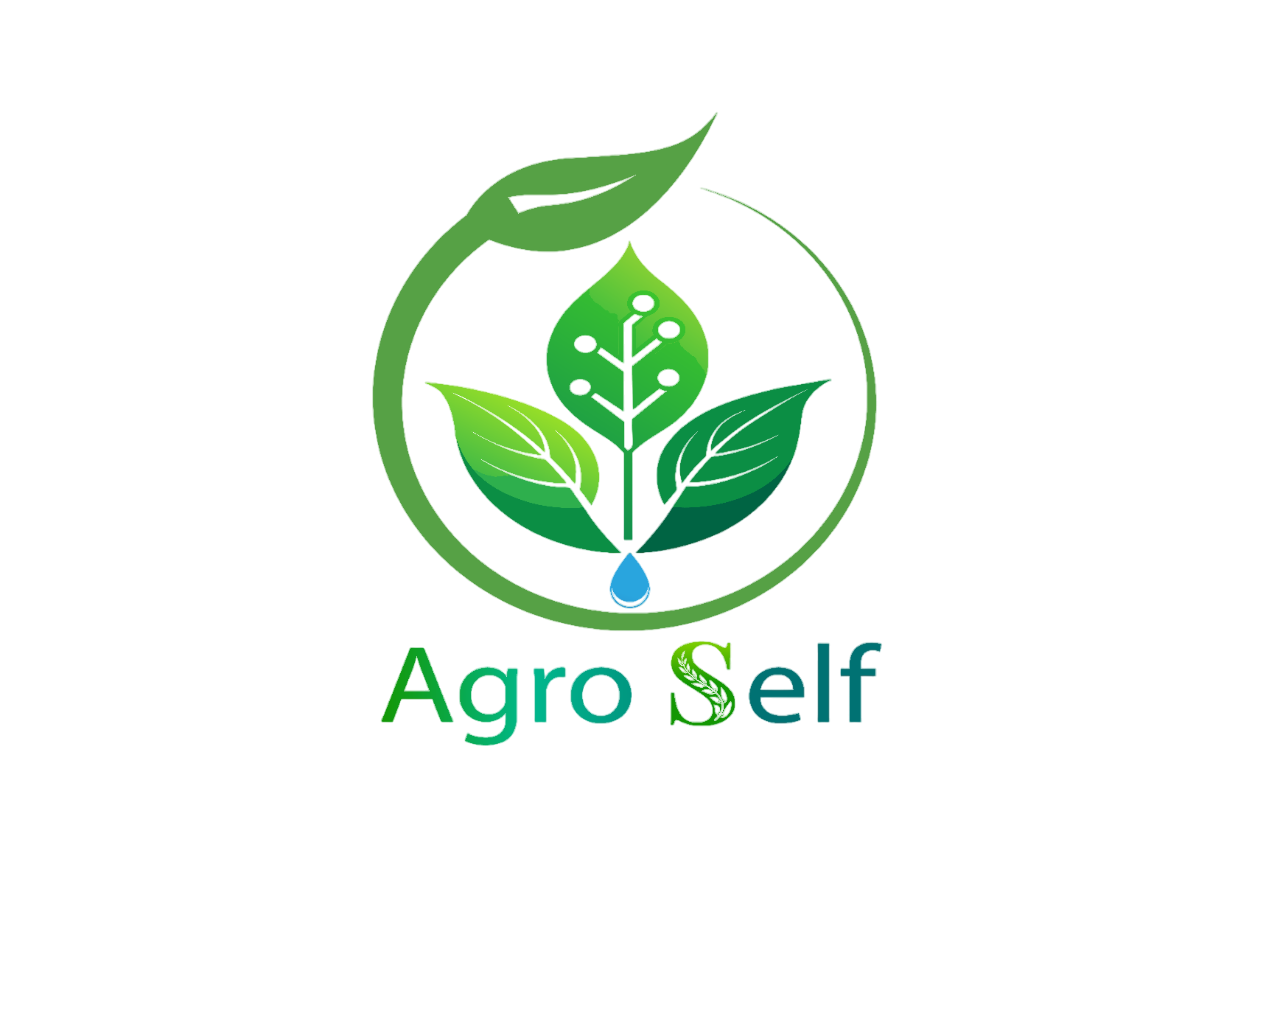
\includegraphics[width=0.95\textwidth]{public/AgroSelf}
\end{minipage}
\hfill 
\begin{minipage}[c]{0.83\textwidth}
	\textbf{AgroSelf: } Solution hydroponique intelligente destinée à l’automatisation de la culture végétale en environnement contrôlé. Le système intègre des mécanismes de surveillance des paramètres climatiques et nutritifs afin d’optimiser la croissance des plantes tout en réduisant la consommation d’eau et d’énergie.
\end{minipage}

\vspace{1cm}  

\noindent
\begin{minipage}[c]{0.12\textwidth}
	\centering
	
\includegraphics[width=0.95\textwidth]{public/grow}
\end{minipage}
\hfill
\begin{minipage}[c]{0.83\textwidth}
	\textbf{GIY (Grow It Yourself): } Solution orientée agriculture domestique et urbaine permettant aux utilisateurs de cultiver des plantes de manière autonome. Elle propose une gestion simplifiée de l’irrigation, de l’éclairage et du suivi de croissance grâce à des technologies connectées adaptées aux petits espaces.
\end{minipage}

\vspace{1cm}  

\noindent
\begin{minipage}[c]{0.12\textwidth}
	\centering
	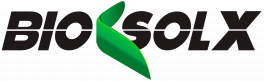
\includegraphics[width=0.95\textwidth]{public/biolo}
\end{minipage}
\hfill
\begin{minipage}[c]{0.83\textwidth}
	\textbf{Biosolx: } Plateforme spécialisée dans les systèmes agricoles intelligents utilisant des capteurs et des solutions IoT pour le contrôle automatisé de l’environnement de culture. Elle vise à améliorer la productivité agricole à travers l’analyse des données en temps réel et la gestion optimisée des ressources.
\end{minipage} \newline


\subsection{Limites des solutions existantes}

Malgré les fonctionnalités avancées offertes par les solutions étudiées, plusieurs limites demeurent présentes. La plupart des solutions reposent fortement sur des infrastructures centralisées ou des services distants, ce qui peut affecter leur autonomie et leur disponibilité. Par ailleurs, les capacités d’intelligence artificielle et de diagnostic automatisé restent souvent limitées ou absentes. Certaines solutions offrent également une faible adaptabilité aux contraintes des exploitations locales et nécessitent des coûts de déploiement ou de maintenance relativement élevés. Le tableau \ref{tab:comparaison-solutions} synthétise les principales limites identifiées à travers l’analyse comparative réalisée.

\begin{table}[!htbp] 
	\centering
	\small
	\renewcommand{\arraystretch}{1.5}
	\begin{tabular}{|p{3.5cm}|p{3.5cm}|p{3.5cm}|p{3.5cm}|}
		\hline
		\rowcolor[HTML]{ECECEC} 
		\textbf{Critères} & \textbf{AgroSelf} & \textbf{GIY (Grow It)} & \textbf{Biosolx} \\ \hline
		
		\textbf{Dépendance Cloud} & Forte dépendance à une infrastructure Cloud pour le contrôle. & Fonctionnement partiellement connecté. & Architecture centralisée dépendante du système distant. \\ \hline
		
		\textbf{Intelligence du système} & Optimisation limitée aux paramètres environnementaux. & Assistance décisionnelle sans autonomie complète. & Automatisation industrielle sans intelligence contextuelle. \\ \hline
		
		\textbf{Vision et diagnostic} & Absence de détection visuelle des maladies. & Observation manuelle par l’utilisateur. & Contrôle basé uniquement sur capteurs physiques. \\ \hline
		
		\textbf{Adaptabilité locale} & Faible adaptation aux environnements ruraux. & Dépendance à la formation utilisateur. & Solution orientée industrie à grande échelle. \\ \hline
		
		\textbf{Coût et accessibilité} & Coût élevé et maintenance complexe. & Coût modéré mais dépendance au support. & Solution industrielle difficilement accessible. \\ \hline

		\textbf{Assistance agronomique} & Aucun accompagnement intelligent à l'agriculteur. & Interface passive sans conseil contextuel. & Pas d'assistance décisionnelle intégrée. \\ \hline
	\end{tabular}
	\caption{Analyse comparative des solutions hydroponiques existantes}
	\label{tab:comparaison-solutions}
\end{table}

L’étude des solutions existantes montre qu’aucune d’entre elles ne répond simultanément aux exigences suivantes : autonomie hors ligne, intégration d’une intelligence artificielle avancée pour le diagnostic biologique, et accessibilité économique adaptée au contexte agricole tunisien.

Ainsi, ces limites justifient la nécessité de proposer une nouvelle architecture plus robuste, autonome et adaptée aux contraintes locales, constituant la base du système développé dans ce projet.


	%----------------------------------------------------------------
\section{ Solution Proposée}
	%----------------------------------------------------------------
	
Pour répondre aux lacunes identifiées, nous proposons le \textbf{HydroNova} : une architecture de contrôle décentralisée et orientée \textit{Edge-first}, conçue pour garantir une résilience opérationnelle totale en mode hors-ligne, tout en tirant parti des capacités d'analyse et de supervision offertes par le Cloud lorsque la connectivité est disponible.

	La solution s'articule autour de quatre axes technologiques complémentaires, avec une priorité stratégique accordée à l'intelligence embarquée :
	
	\begin{itemize}
		\item \textbf{L’Intelligence Artificielle Embarquée (Cœur de la détection sanitaire) :} Véritable pilier de la solution, ce module repose sur un réseau de neurones convolutifs (CNN) spécifiquement entraîné pour le diagnostic phytosanitaire du fourrage hydroponique. Déployé directement sur le Raspberry Pi sous forme d'un modèle quantifié en format ONNX (FP16), il effectue une inférence locale pour identifier en temps réel les marqueurs précoces de moisissures ou de stress fongique sur les images capturées par la caméra intégrée. Le traitement s'opère intégralement en local, garantissant une latence quasi nulle et une disponibilité totale indépendante de l'état du réseau. Cette sentinelle numérique assure une vigilance sanitaire permanente, capable d'isoler une menace biologique avant même qu'elle ne soit perceptible à l'œil nu.
		
		\item \textbf{Le Contrôleur Edge Autonome (Raspberry Pi) :} Ce nœud de calcul central exécute des services multi-processus optimisés assurant la régulation déterministe du microclimat : température, hygrométrie, pH, cycles d'irrigation et éclairage artificiel. Un mécanisme de surveillance matérielle de type Watchdog garantit le redémarrage automatique de tout service défaillant, préservant ainsi l'intégrité biologique de la culture contre tout arrêt non prévu du système.
		
		\item \textbf{Backend et Gestion de Données :}  L'orchestration globale est assurée par une architecture robuste développée sous Spring Boot selon les principes de la Clean Architecture. Ce centre de commandement gère la réception asynchrone des flux télémétriques via le protocole sécurisé MQTTS, et ingère les données dans InfluxDB, une base de données spécialisée dans le stockage et l'analyse efficace des séries temporelles. Cette couche analytique transforme les relevés bruts en historiques exploitables pour l'optimisation continue des rendements. Un chatbot agronomique basé sur une architecture RAG (Retrieval-Augmented Generation) avec Gemini complète ce dispositif en offrant un accompagnement intelligent et contextualisé à l'agriculteur.
		\item \textbf{Interfaces de Supervision :}  L'interaction avec les utilisateurs est assurée par deux interfaces complémentaires. L'application mobile développée sous Flutter permet un pilotage nomade de la serre et la réception immédiate d'alertes critiques. Le tableau de bord d'administration React, associé à Grafana, offre aux gestionnaires une vue analytique haute résolution de l'ensemble du parc, avec configuration à distance et visualisation des séries temporelles.
	\end{itemize}
	En s'appuyant sur du matériel libre (Raspberry Pi) et des logiciels open-source, cette architecture réduit significativement les coûts d'acquisition et de maintenance, la rendant accessible aux exploitations de taille moyenne dans le contexte agricole tunisien. En combinant l'autonomie de l'Edge Computing aux capacités d'analyse du Cloud, cette solution vise à transformer la culture hydroponique en un processus sécurisé, intelligent et économiquement viable.
	% Positionnement de la figure immédiatement après la description

% ---------------------------------------------------------------
\section{Méthodologie de gestion de projet}
%----------------------------------------------------------------

La réussite d’un projet multidisciplinaire tel que \textit{HydroNova} repose non seulement sur les choix technologiques, mais aussi sur l’adoption d’une méthodologie de gestion adaptée à la nature hybride du système. Ce projet combine en effet plusieurs dimensions complémentaires : des composants matériels (capteurs, actionneurs, Raspberry Pi, Arduino), des communications IoT temps réel (MQTT), un module d’intelligence artificielle (inférence locale CNN, assistant VLM cloud), un backend centralisé (Spring Boot, bases de données) et des interfaces utilisateurs multiples (Flutter, React).

Le projet \textit{HydroNova} présente trois caractéristiques majeures qui justifient le recours à plusieurs méthodes:

\begin{enumerate}
	\item \textbf{Intégration matérielle et logicielle}: Le système comporte une partie embarquée critique (contrôle des actionneurs, acquisition des capteurs) qui doit respecter des contraintes de temps réel et de fiabilité. Cette partie nécessite une validation formelle et une traçabilité rigoureuse.
	\item \textbf{Développement logiciel distribué}: Le backend, l’application mobile et le tableau de bord web évoluent de manière continue. Ils appellent une gestion de flux flexible, capable de s’adapter aux changements sans bloquer l’intégration.
	\item \textbf{Module d’intelligence artificielle}: La détection des maladies repose sur des données et des modèles d’apprentissage. Ce volet exige un cycle itératif spécifique (compréhension des données, préparation, modélisation, évaluation) différent du cycle classique du génie logiciel.
\end{enumerate}

Aucune méthode unique ne couvre l’ensemble de ces exigences. Une approche méthodologique composite s’impose, où chaque sous‑système est piloté par la méthode la mieux adaptée à son domaine, le tout étant orchestré par un \textbf{cadre global en V} qui garantit la traçabilité et la cohérence d’ensemble.

%----------------------------------------------------------------
\subsection{Présentation synthétique des méthodes retenues}
%----------------------------------------------------------------

\subsubsection*{Modèle en V}
Organisé en deux branches symétriques (spécification descendante, validation ascendante), il assure une traçabilité complète entre les exigences et les tests. Chaque phase de conception est associée à une phase de vérification de même niveau. Ce modèle est particulièrement adapté aux systèmes embarqués critiques et à l’intégration matérielle.
%\begin{figure}[!htbp]
%	\centering
%	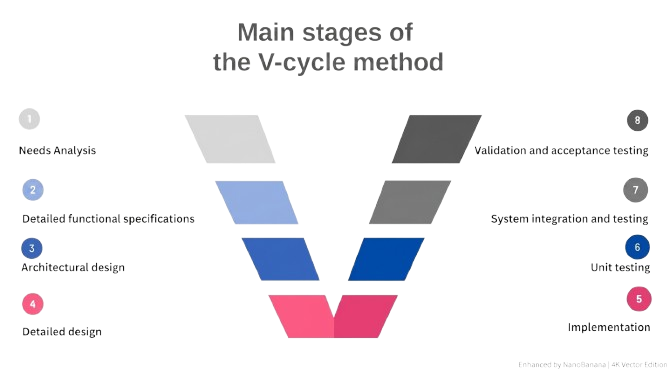
\includegraphics[width=0.75\linewidth]{public/vmodelpp}
%	\caption{Le modèle en V — phases de conception et de validation en symétrie}
%	\label{fig:vmodelpp}
%\end{figure}

\subsubsection*{Kanban}
%\begin{figure}[h!]
%	\centering	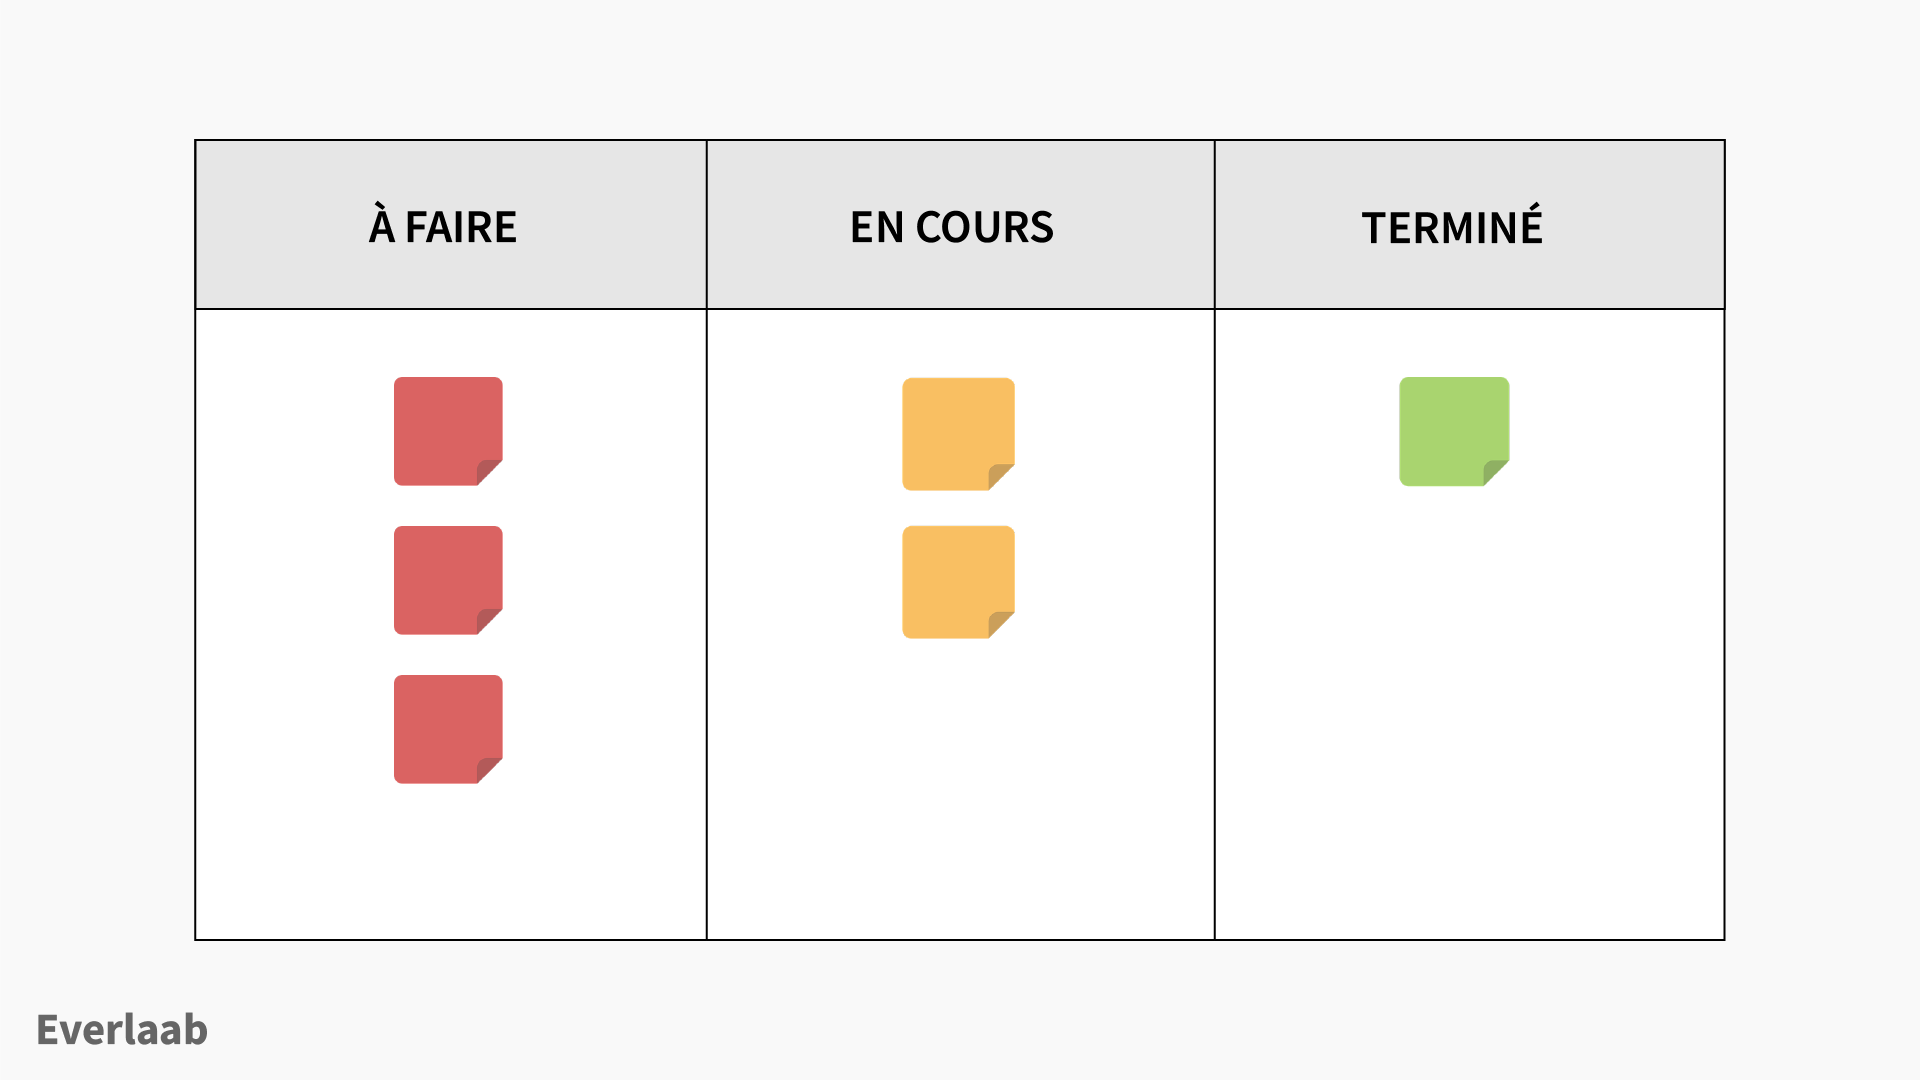
\includegraphics[width=0.75\linewidth]{public/kanban-1}
%	\caption{Fonctionnement du tableau Kanban — flux de tâches par colonnes}
%	\label{fig:kanban-1}
%\end{figure}
Méthode de gestion visuelle du travail en flux continu. Elle repose sur un tableau divisé en colonnes (À faire, En cours, Terminé) et sur une limitation du travail en cours (WIP). Kanban permet une grande flexibilité pour les tâches de développement logiciel et s’intègre facilement à d’autres cadres.


\subsubsection*{CRISP-DM}
Cadre de référence pour les projets d’intelligence artificielle. Il définit six phases itératives (compréhension du domaine, compréhension des données, préparation, modélisation, évaluation, déploiement). Ce cycle permet de revenir en arrière lorsque les résultats d’un modèle sont insuffisants.
\begin{figure}[!htbp]
	\centering
	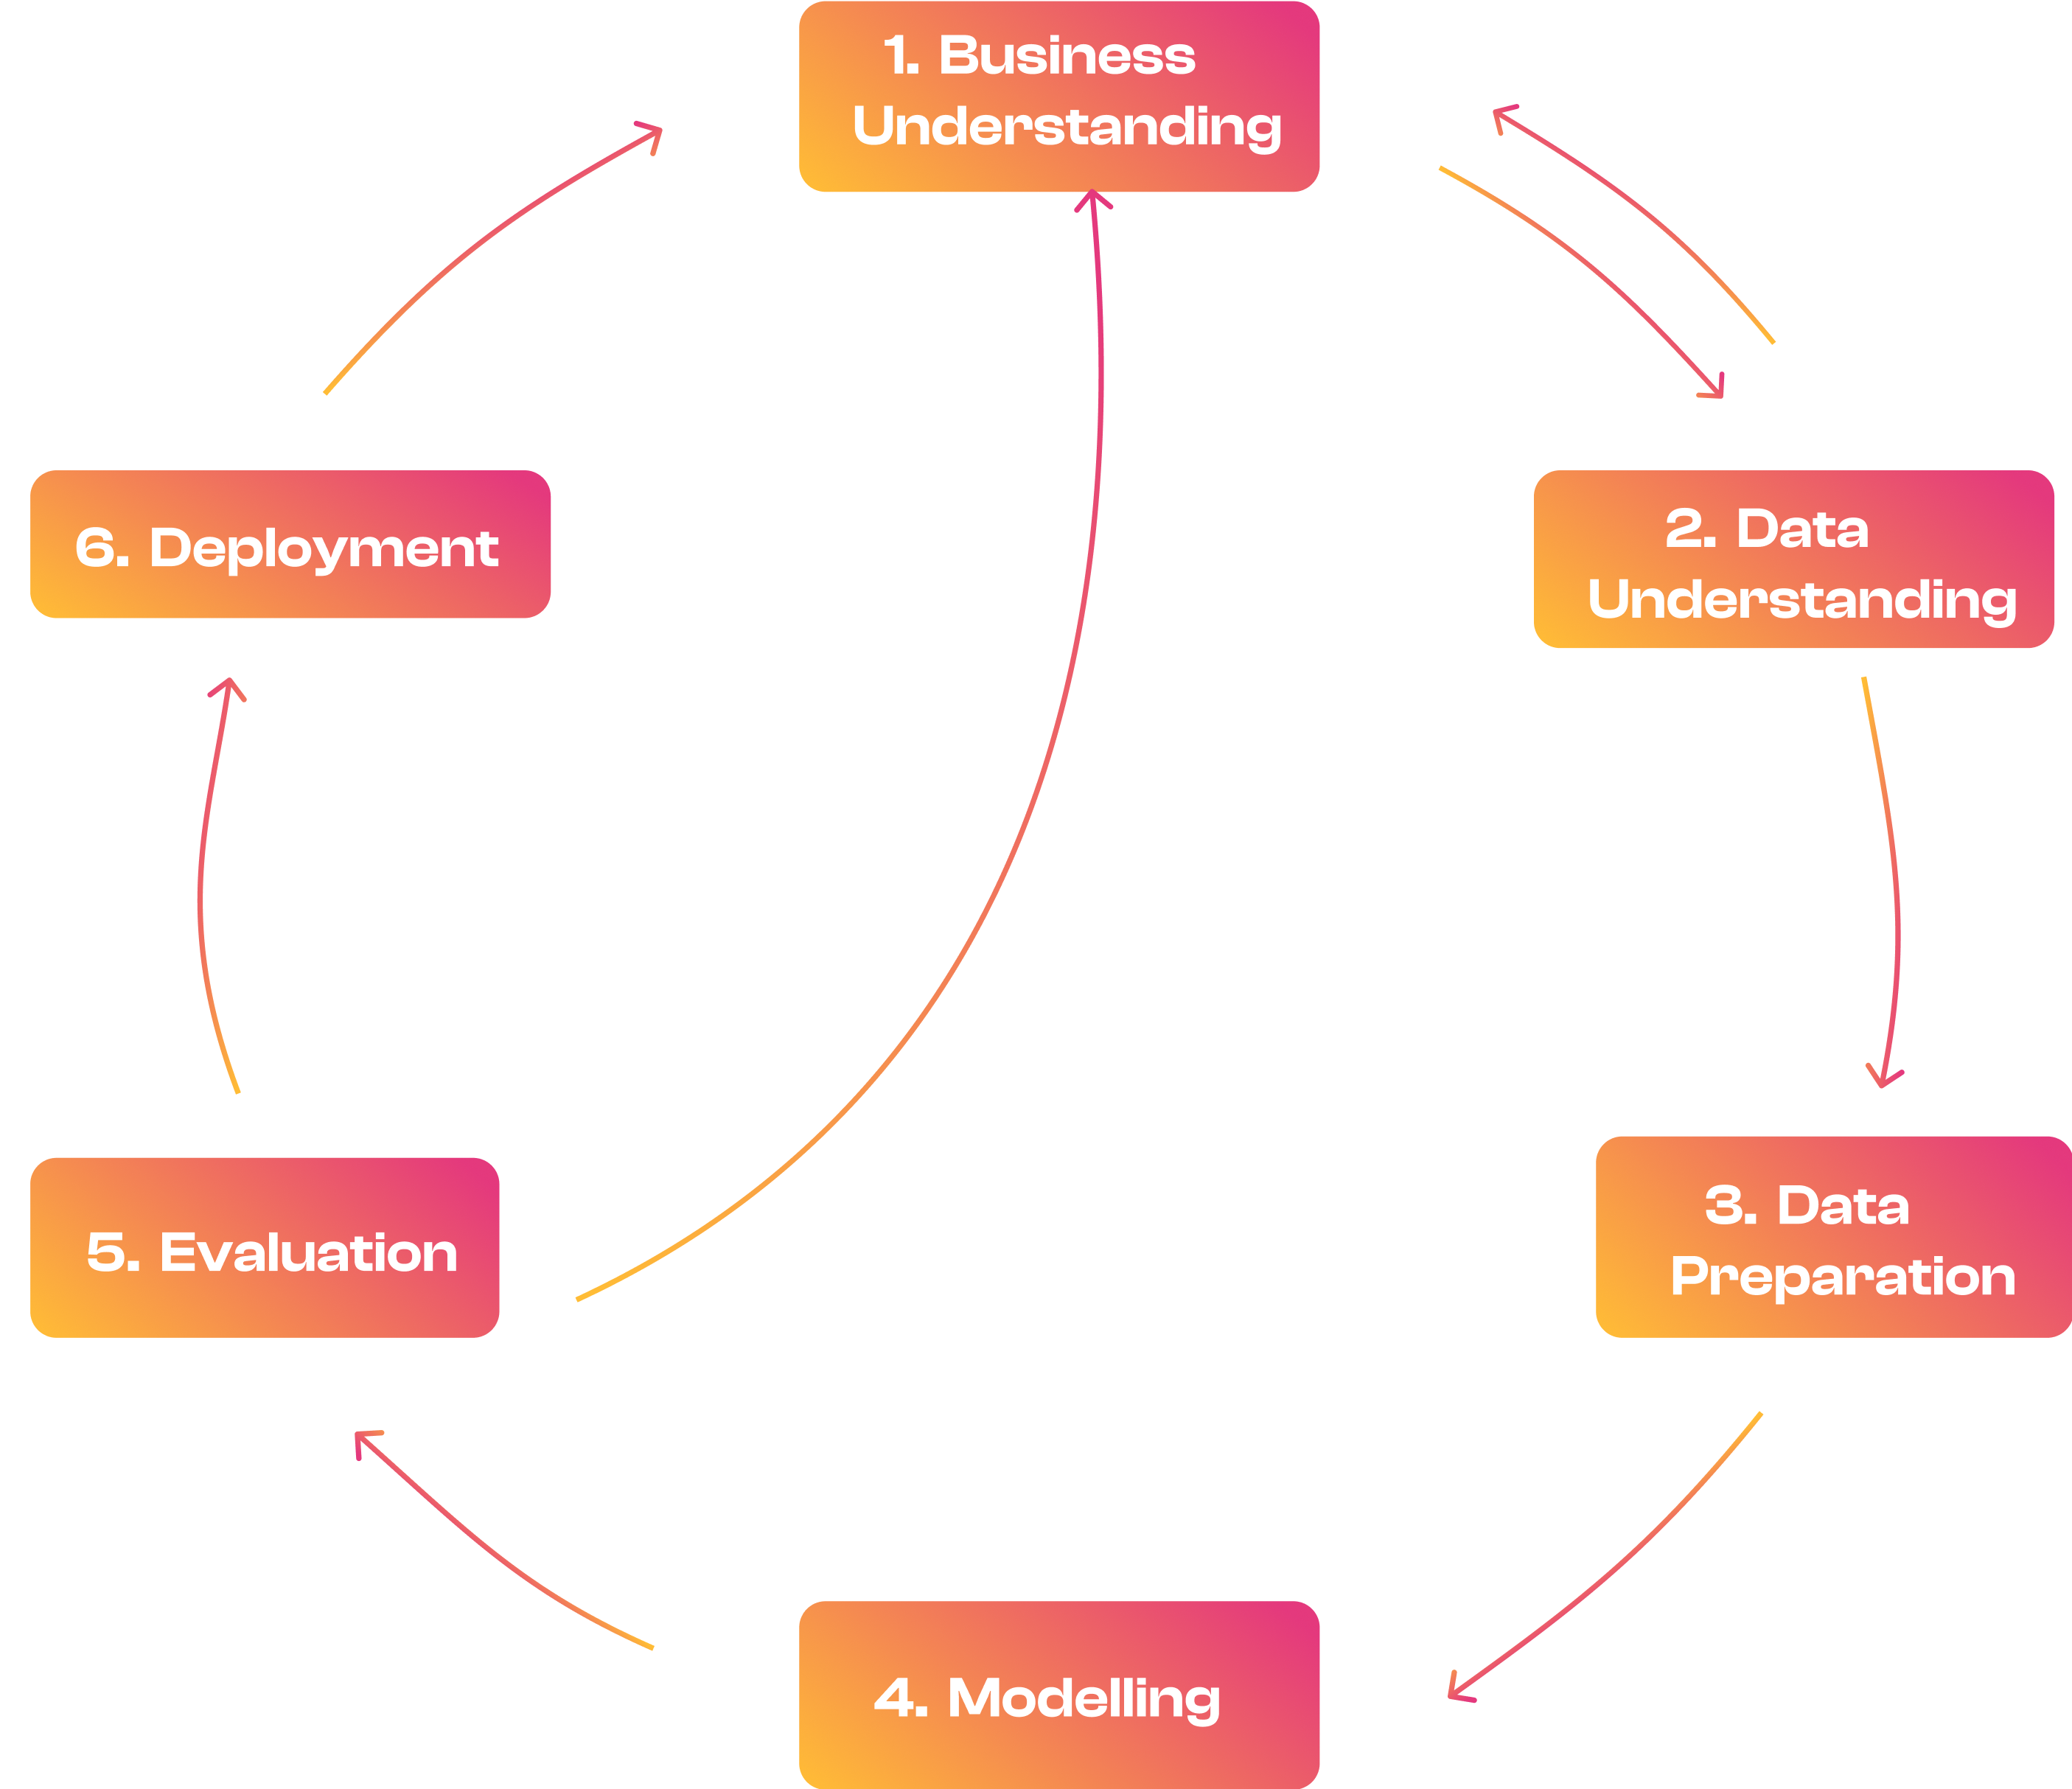
\includegraphics[width=0.6\linewidth]{public/crispdm}
	\caption{Le cycle CRISP-DM — six phases itératives pour les projets IA}
	\label{fig:crispdm}
\end{figure}

Ces trois approches présentent des profils complémentaires, comme le résume le tableau~\ref{tab:comparaison_methodologies}.

\begin{table}[!htbp]
	\centering
	\small
	\renewcommand{\arraystretch}{1.5}
	\begin{tabularx}{\textwidth}{|p{0.28\textwidth}|X|X|X|}
		\hline
		\rowcolor[HTML]{2C3E50}
		\textcolor{white}{\textbf{Critère}} & \textcolor{white}{\textbf{Kanban}} & \textcolor{white}{\textbf{Cycle en V}} & \textcolor{white}{\textbf{CRISP-DM}} \\ \hline
		\rowcolor[HTML]{EFEFEF}
		Gestion des projets IoT & Bon & Excellent & Faible \\ \hline
		Développement logiciel & Excellent & Bon & Faible \\ \hline
		\rowcolor[HTML]{EFEFEF}
		Gestion des systèmes embarqués & Moyen & Excellent & Faible \\ \hline
		Traçabilité & Moyen & Excellent & Moyen \\ \hline
		\rowcolor[HTML]{EFEFEF}
		Flexibilité & Excellent & Faible & Bon \\ \hline
		Validation formelle & Moyen & Excellent & Moyen \\ \hline
		\rowcolor[HTML]{EFEFEF}
		Projets IA & Bon & Moyen & Excellent \\ \hline
	\end{tabularx}
	\caption{Comparaison des méthodologies étudiées}
	\label{tab:comparaison_methodologies}
\end{table}

%----------------------------------------------------------------
\subsection{Hybridation au sein du modèle en V}
%----------------------------------------------------------------

Le cadre global du projet est le modèle en V. Il structure le rapport et le déroulement du projet, depuis l’analyse des besoins (chapitre III) jusqu’aux tests de validation (chapitre VI). Cependant, à l’intérieur de certaines phases du V, d’autres méthodes sont utilisées pour répondre aux spécificités des composants.

\begin{itemize}
	\item \textbf{Phase de conception détaillée}: Pour le module IA, au lieu d’une spécification linéaire, nous exécutons un cycle CRISP-DM complet (compréhension des données, préparation, modélisation, évaluation). Ce cycle est itéré localement jusqu’à l’obtention d’un modèle satisfaisant. Une fois figé, le modèle entre dans la phase de réalisation du V.
	\item \textbf{Phase de réalisation et implémentation}: Le développement du backend, de l’application mobile et de l’interface web est géré par \textbf{Kanban} : un tableau numérique suit les tâches en flux continu, avec limitation du travail en cours (WIP). Les tâches sont découpées finement et intégrées dès qu’elles sont terminées, sans attendre la fin d’un sprint.
	\item \textbf{Branche ascendante (validation)}: Les tests d’intégration et les tests système respectent strictement le modèle en V, mais ils intègrent des boucles de rétroaction: par exemple, une anomalie détectée lors des tests d’intégration MQTT remonte vers la spécification des exigences pour affiner la QoS.
\end{itemize}

La figure~\ref{fig:hybridation_v} illustre cette hybridation : le V global contient des « poches » méthodologiques où Kanban et CRISP-DM s’exécutent de manière itérative ou continue, tout en restant raccordées aux jalons du V.

\begin{figure}[!htbp]
	\centering
	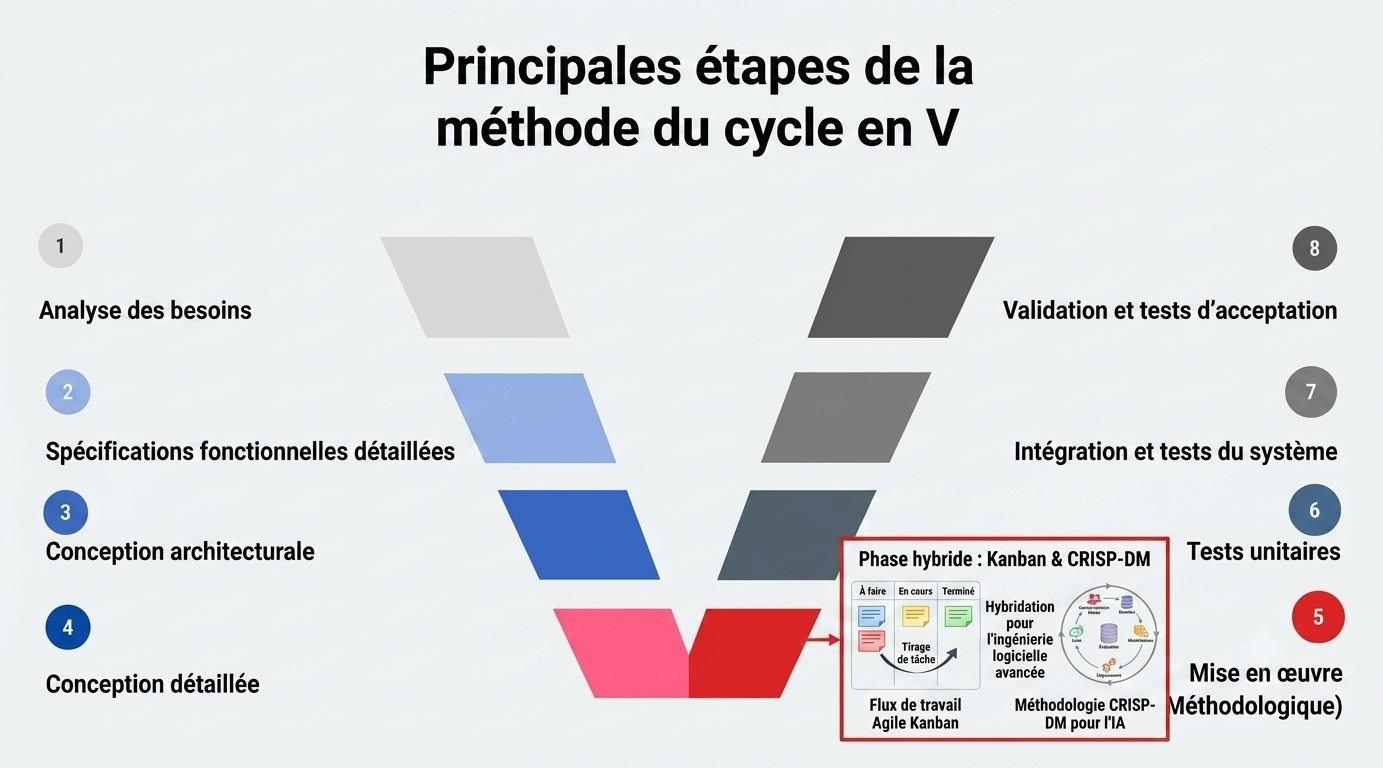
\includegraphics[width=0.85\linewidth]{public/methaoly}
	\caption{Hybridation méthodologique : Kanban et CRISP-DM imbriqués dans le Cycle en V}
	\label{fig:hybridation_v}
\end{figure}

L’hybridation n’est pas un empilement arbitraire : elle repose sur une analyse précise des forces et limites de chaque méthode (tableau~\ref{tab:comparaison_methodologies}). Le modèle en V fournit le squelette — il fixe les jalons majeurs et assure la traçabilité ascendante/descendante. À l’intérieur de ce squelette, CRISP-DM apporte l’itération nécessaire à la fouille de données, tandis que Kanban apporte la fluidité pour le développement logiciel.
Le tableau~\ref{tab:methodologies_composantes} détaille l’affectation de chaque composant ou phase à la méthode principale, tout en précisant comment l’hybridation est mise en œuvre. 

\begin{table}[!htbp]
	\centering
	\small
	\renewcommand{\arraystretch}{1.5}
	\begin{tabularx}{\textwidth}{|p{6.5cm}|X|}
		\hline
		\rowcolor[HTML]{2C3E50}
		\textcolor{white}{\textbf{Phase / Activité}} & \textcolor{white}{\textbf{Méthodologie appliquée}} \\ \hline
		\rowcolor[HTML]{EFEFEF}
		Analyse des besoins (chapitre II) & Cycle en V (cadre) \\ \hline
		Conception architecturale (chapitre III) & Cycle en V \\ \hline
		\rowcolor[HTML]{EFEFEF}
		Conception détaillée IA & CRISP-DM (itératif, intégré dans la phase de conception du V) \\ \hline
		Développement Backend (Spring Boot) & Kanban \\ \hline
		\rowcolor[HTML]{EFEFEF}
		Développement Mobile (Flutter) & Kanban \\ \hline
		Développement Interface Web (React) & Kanban \\ \hline
		\rowcolor[HTML]{EFEFEF}
		Système IoT et firmware (Arduino / Raspberry Pi) & Cycle en V  \\ \hline
		Intégration globale & Cycle en V \\ \hline
		\rowcolor[HTML]{EFEFEF}
		Validation et tests (chapitre V) & Cycle en V \\ \hline
	\end{tabularx}
	\caption{Application des méthodologies aux différentes composantes du projet}
	\label{tab:methodologies_composantes}
\end{table}

	
	\section*{Conclusion}
\addcontentsline{toc}{section}{Conclusion}

Ce premier chapitre a posé les bases du projet \textit{HydroNova} en présentant son contexte institutionnel, son environnement technologique et la méthodologie de gestion retenue. L’analyse des solutions agricoles intelligentes existantes a révélé plusieurs limitations récurrentes, notamment une forte dépendance à la connectivité Internet et aux infrastructures Cloud, ce qui restreint leur déploiement dans les zones rurales peu desservies et expose les exploitants à des risques de latence ou de panne réseau.

Ces constats justifient la conception d’une architecture originale, résiliente et capable de fonctionner en mode hors ligne, où l’intelligence est répartie entre la périphérie (Edge AI sur Raspberry Pi) et le Cloud, et où les décisions critiques sont prises localement.

Par ailleurs, l’adoption d’une approche méthodologique hybride, combinant le Cycle en V pour la rigueur et la traçabilité, Kanban pour la fluidité du développement logiciel, et CRISP‑DM pour l’itération propre à l’intelligence artificielle. Cette hybridation offre un cadre de développement à la fois structuré, flexible et adapté aux spécificités d’un projet intégrant des composantes matérielles, logicielles et IA.

Les fondements du projet étant désormais établis, le chapitre suivant entre dans la phase d’étude approfondie. Il sera consacré à un état de l’art des architectures et méthodes intelligentes appliquées au domaine agricole. Nous y examinerons les techniques d’intelligence artificielle pour la détection de maladies végétales (CNN, Vision-Language Models, apprentissage par ensemble). Cette analyse permettra de positionner les choix technologiques d’\textit{HydroNova} par rapport aux travaux antérieurs et de justifier les orientations retenues pour la suite du projet.
